\subsection{from Smith}

The discovery of Physics Beyond the Standard Model (BSM) is the main target of
current high energy experiments. One way to search for this New Physics is to
measure precisely some low energy parameters, in the hope of observing a
deviation with respect to the Standard Model (SM) prediction. In this respect,
CP violation is particularly interesting because in the SM, it originates from
a single parameter. All the CP violating observables in the $K$, $B$ and $D$
meson sectors are thus related and their combined study provides a highly
powerful test of the whole SM dynamics. By contrast, most model of New Physics
are far less restrictive and allow for a plethora of new CP-violating sources.
None of the delicate interplays between observables expected in the SM should
survive to the presence of new dynamics at the~TeV scale. In this respect, one
activity of the French community, the CKM fitter collaboration, is precisely
to test the coherence of CP violation measurements. It is embodied in the well
known Unitary Triangle (UT), a consequence of the unitarity of the CKM matrix
in the SM. In the absence of New Physics, its sides and angles as determined
from various observables all have to agree for the triangle to close.

When experimentally testing SM predictions, it is fundamental that the
theoretical precision matches the experimental accuracy. A priori, this looks
challenging because CP-violation is a purely hadronic phenomenon in the SM,
originating from the quark couplings. However, dedicated strategies have been
designed and CP-violating observables are actually among our best windows. For
example, in CP-violating asymmetries, most of the uncertainties cancel between
the numerator and the denominator, so that we can construct measurable
quantities with small uncertainties. Alternatively, some observables are
predicted to be so small that they can be considered forbidden in the SM, and
simply observing a non-zero value would unequivocally signal the presence of
New Physics.

The French community has been deeply involved in various key CP-violation
experiments for many years (CPLEAR, NA48, BaBar, LHCb, ...). Let us describe
briefly the current status and some activities planned in the near future.

\subsubsection*{CP-violation in the $B$ sector}

The French community has developed a recognized expertise in several key
aspects of the study of CP-violation: amplitude analyses, tagged
time-dependent angular analyses, flavour tagging, neutral objects, ... More
specifically, we have been involved in the measurements of the UT angles
$\alpha$, $\gamma$ and $\phi_{s}$. The following decays channels have been
studied in details: $B^{0}\rightarrow\rho\rho$, $B_{(s,d)}\rightarrow
K_{\mathrm{S}}^{0}hh$, $B_{(s,d)}\rightarrow D^{0}K^{\ast0}$, $B_{(s,d)}%
\rightarrow\bar{D}^{0}hh$, $B_{s}^{0}\rightarrow D_{s}K$, $B^{0}\rightarrow
K_{\mathrm{S}}^{0}K\pi$, $B_{s}^{0}\rightarrow J/\psi\phi$, $B_{s}%
^{0}\rightarrow J/\psi\bar{K}^{\ast0}$. One of the outcome of the work done in
$\phi_{s}$ is illustrated on Figure~\ref{figphis}. Besides, it should be
mentioned that we have been in charge of designing, building and maintaining
key elements of the detectors (trigger and calorimeters).

In the coming years, most of the experimental effort will go in LHCb and its
upgrade plans. One of the biggest challenge will be to store and analyse the
enormous quantity of data from the LHC. In the 2017-2020 time span, we will
not only continue the measurements started many years ago, with the full run2
data-set of the LHC, but also explore new routes:

\begin{itemize}
\item Several ways to measure $\gamma$ and $\alpha$ to overconstrain the UT;

\item Continue efforts on $\phi_{s}$ and control of subleading penguin contributions;

\item Explore CP violation in bottom baryons;

\item Actively participate to the brainstorming on future upgrade of the LHCb
experiment, i.e. plans for the 2025-2035 period.
\end{itemize}

For all these items, the synergy between experimental and theoretical
communities is essential because a major discovery cannot come if the
uncertainties are not under control in both places. Advances in controlling
hadronic effects, for example using lattice simulations of QCD or analytic
tools like sum rules can be expected.

\subsubsection*{CP-violation in the $D$ and $K$ sectors}

For a complete picture of CP violation, and to test the CKM paradigm, CP
violation in $K$ and $D$ physics should be studied in parallel to that in $B$
physics. More specifically:

\begin{itemize}
\item Kaon physics is the birthplace of CP violation, and has played a central
role in establishing the CKM picture in the past five decades. Currently, two
main aspects are relevant for our proposed plans. First, advances in lattice
QCD may help to finally shed new light on the precisely measured direct
CP-violation parameter $\varepsilon^{\prime}$. Second, theorists will be
following closely the NA62 experiment which aims at $K^{+}\rightarrow\pi
^{+}\nu\nu$. Any hint of discrepancy with the SM there would have implications
for the other meson sectors.

\item Theoretically, CP violation in charm mesons is expected to be very small
because the GIM mechanism is much more powerful for $c\rightarrow u$
transitions than for $s\rightarrow d$ or $b\rightarrow s,d$ transitions. At
the same time, New Physics need not respect this peculiar feature, so these
observables provide interesting windows for the future and are in the scope of
LHCb measurements.
\end{itemize}

\subsubsection*{CP-violation in other observables}

In the SM, CP violation is a purely flavored phenomenon, arising from the
presence of three families of matter particles. This partly explains its
strong suppression in physical observables, and thereby their high sensitivity
to non-standard sources of CP violation. At the same, this feature is not
fully understood and raises several questions:

\begin{itemize}
\item CP violation by the strong interaction is mysteriously absent from the
SM. If present, it would deeply alter the picture, in particular for electric
dipole moments. This is the so called strong CP problem. In this context, the
French community is actively involved in the next generation of neutron EDM experiments.

\item The study of CP violation could have deep cosmological consequences. For
example, one solution to the strong CP problem involves a new particle, the
axion, whose relic density could play a role in the context of dark matter.
Another puzzle is the origin of the baryon asymmetry of the Univerve, which
seems to require some new sources of CP violation.
\end{itemize}

Thus, exploring CP violation in light mesons has implications well beyond the
strict context of flavor physics, and may shed new lights on some of the most
fundamental puzzles.

\begin{figure}[ptb]
\begin{center}
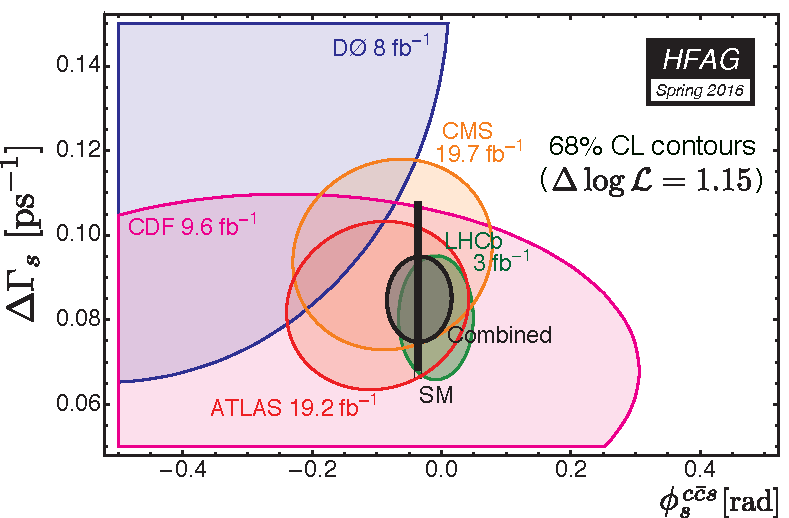
\includegraphics[width=10cm]{hfag_Spring2016_DGsphis_zoom.pdf}
\end{center}
\caption{68\% CL regions in $B^{0}_{s}$ width difference $\Delta\Gamma_{s}$
and weak phase $\phi_{s}$ obtained from individual and combined CDF, D0,
ATLAS, CMS and LHCb likelihoods of $B^{0}_{s}\to J/\psi\phi$, $B^{0}_{s}\to
J/\psi KK$, $B^{0}_{s}\to J\psi\pi\pi$ and $B^{0}_{s}\to D_{s}^{+}D_{s}^{-}%
$.The expectation within the Standard Model is shown as the black rectangle.}%
\label{figphis}%
\end{figure}

%\end{document}